\chapter{The Neural Network used for signal-background classification}
\section{Short introduction to neural networks}
Neural networks are loosely on the human brain and are a means of doing machine learning, in which a computer learns to perform some task by analyzing training examples. 
A NN is usually organized into layers of processing nodes. These processing nodes are densely interconnected between layers, and every connection weighted. 
During the $forward$ $propagation$, where the NN is tested on provided data, computations in the NN propagate from the input layer to the output layer. An individual node receives data from nodes in the layer beneath it and sends data to nodes in the layer above. 
Nodes multiply received data by their weight value and add them together to a single value. Only if the node exceeds a specific threshhold does it send its value to the next layer. During $backpropagation$, where the NN is being trained, weights and thresholds are continually adjusted until training data with the same label yield similar results.   
In this thesis, a NN discriminates between the $tq\gamma$ signal and background events. 
The NN is trained on Monte Carlo simulations (Section \ref{sec:mc}) and is tested on measurement data after that. Characteristic variables of events, which are discussed in detail in section \ref{sec:inputfeatures}, are used as the input. 
\section{The neural network architecture}
\label{sec:arch}
The NN are built using the \texttt{Keras} library running on \texttt{TensorFlow} \cite{Keras} \cite{tensorflow}.
Two different neural networks are trained to separate the signal from the background. One is trained on the zero-forward jet signal region ($0\text{-}fj$), and the other is trained on the At least one forward jet region ($\geq 1\text{-}fj$). 
This is done to optimize the sensitivity of the analysis as the signal to background ratio ($S/B$) is greater for the $\geq 1\text{-}fj$ region than the $0\text{-}fj$ region. \\
Both models consist of one input layer, three densely connected node layers (Dense layer) and one output layer. The input layers have nodes for each input feature. The NN for $0\text{-}fj$ events has $16$ input features while the NN for $\geq 1\text{-}fj$ events has $27$ due to additional variables of the forward jets. 
The activation function for the Dense layers is the Leaky Rectified Linear Unit (ReLU) function $f(x)$:
\begin{align*}
    f(x) =\begin{cases}
            x, & \text{for } x \geq 0\\
            0.5x, & \text{for } x < 0.
        \end{cases}
\end{align*}
For the output layer, the activation function is the sigmoid function $\sigma(x)$:
\begin{align*}
    \sigma(x) = \frac{1}{1+ e^{-x}}. 
\end{align*}
Finally, the \texttt{Adam} algorithm is used as the optimizer for updating the weights in the NN \cite{Adam}. Figure \ref{fig:models} displays the described architecture of the NN models. 
\begin{figure}
    \centering
    \begin{subfigure}{.5\textwidth}
      \centering
      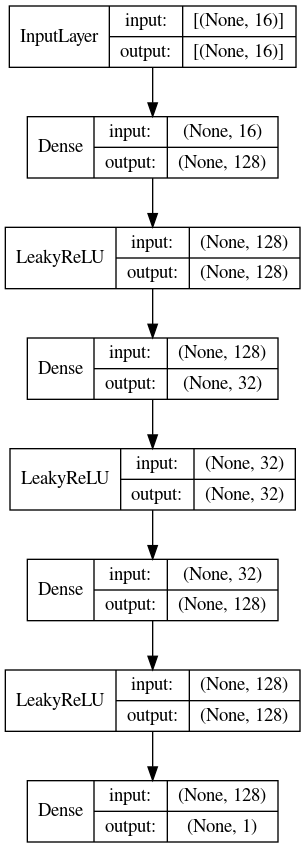
\includegraphics[width=.4\linewidth]{Plots/model_0fj.png}
    \end{subfigure}%
    \begin{subfigure}{.5\textwidth}
      \centering
      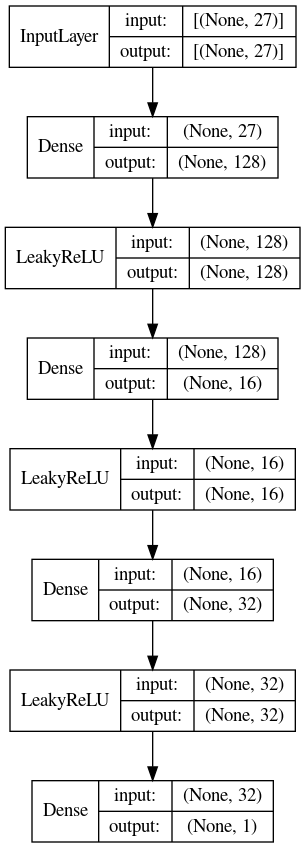
\includegraphics[width=.4\linewidth]{Plots/model_1fj.png}
    \end{subfigure}
    \caption{Visualization of the NN architecture for the zero forward jet region (left) and the $\geq 1$ forward jets region (right).}
    \label{fig:models}
\end{figure}

\section{Input features for the neural network}
\label{sec:inputfeatures}
The input features used for the two NN models are listed in table \ref{tab:features} (Weiß nicht was ich hier schreiben sollte?).
\begin{table}
    \centering
    \begin{tabular}{c|c|c}
        \toprule
        {} &                     0fj variables      & 1fj variables\\
        \midrule 
        1  &                                HT      & HT\\ \hline
        2  &                           blep\_dr     & blep\_dr\\ \hline
        3  &                           lbj\_eta     &lbj\_eta\\ \hline
        4  &                            lbj\_pt     &lbj\_pt\\ \hline
        5  &  lbj\_tagWeightBin\_DL1r\_Continuous   & lbj\_tagWeightBin\_DL1r\_Continuous\\ \hline
        6  &                          lep1\_eta     & lep1\_eta\\ \hline
        7  &                           met\_met     &met\_met\\ \hline
        8 &                             ph\_pt     &ph\_pt\\ \hline
        9 &                             top\_m     & top\_m\\ \hline
        10 &                       transMassWb      &transMassWb\\ \hline
        11  &                            bph\_pt     & bph\_m\\ \hline
        12 &                          topph\_pt     &topph\_ctheta\\ \hline
        13 &                            ph\_eta     & ph\_phi\\ \hline
        14 &                          lepph\_dr     & lep1\_pt\\ \hline
        15 &                      transMassWph      & met\_phi\\ \hline
        16 &                           lep1\_id     & lbj\_phi\\ \hline
        17 &&                                           Wbsn\_e \\ \hline
        18 &&                                            bfj\_m \\ \hline
        19 &&                                           blep\_m \\ \hline
        20 &&                                           fj\_eta \\ \hline
        21 &&                                           fj\_phi \\ \hline
        22 &&                                        fjet\_flag \\ \hline
        23 &&                                      fjph\_ctheta \\ \hline
        24 &&                                        fjph\_deta \\ \hline
        25 &&                                          fjph\_dr \\ \hline
        26 &&                                           fjph\_e \\ \hline
        27 &&                                           fjph\_m \\ \hline
        \bottomrule 
    \end{tabular}
    \caption{Input variables of the NN trained on events with no forward jets and the NN trained on events with at least one forward jet.}
    \label{tab:features}
\end{table}


\section{Performance and distribution of the NN output}
A distribution for ten different bins of the NN output for $\geq 1\text{-}fj$ has been calculated and displayed in figure \ref{fig:NNdistro}. In this plot, the contributions from different samples are labeled and stacked on top of each other. The data samples are viewed seperately and also added to the plot.
To better visualize the composition of different bins, the right plot in figure \ref{fig:NNdistro} shows the percentage of each sample in each bin. These plots confirm that events at higher values of the NN output increase the $S/B$ ratio.  \\ 
To determine the performance of the NN output, the signal efficiency is plotted alongside the background suppression (so-called "ROC-Curve") in figure \ref{fig:rocfull}. 
The signal efficiency (SE) is calculated as follows: 
\begin{align*}
    SE = \frac{\text{Amount of true signal events }}{\text{Total of signal events}} & \text{Wie schreibe ich das besser?}
\end{align*}
and the background suppression (BS) is calculated with the formula
\begin{align*}
    BS = 1 - \frac{\text{Amount of true background events }}{\text{Total of background events}} & \text{Wie schreibe ich das besser?}.
\end{align*}




\begin{figure}
    \centering
    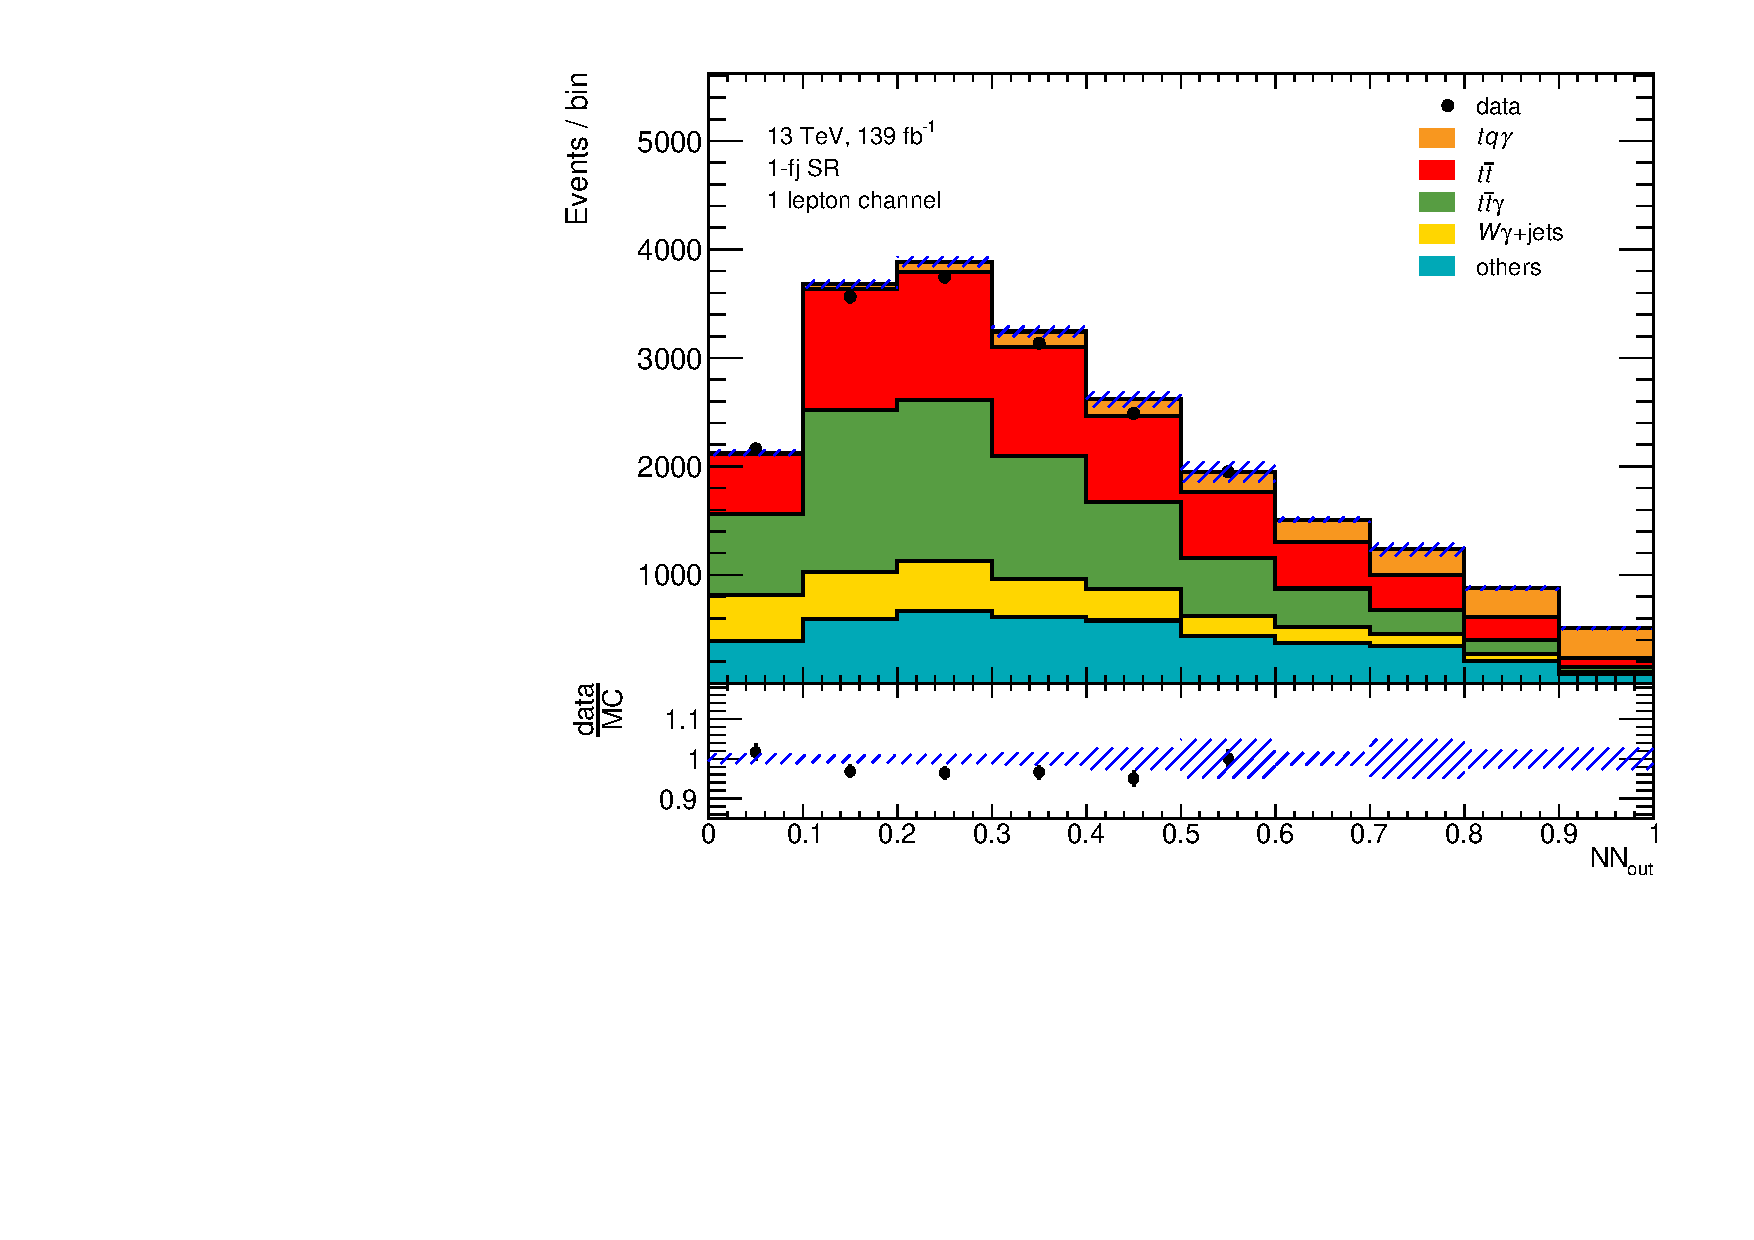
\includegraphics[width=0.8\textwidth]{Plots/NN_out_mix_GANZ.pdf}
    \caption{The NN output event distribution (left) and the composition of different bins of the NN output (right).}
    \label{fig:NNdistro}
\end{figure}
\begin{figure}
    \centering
    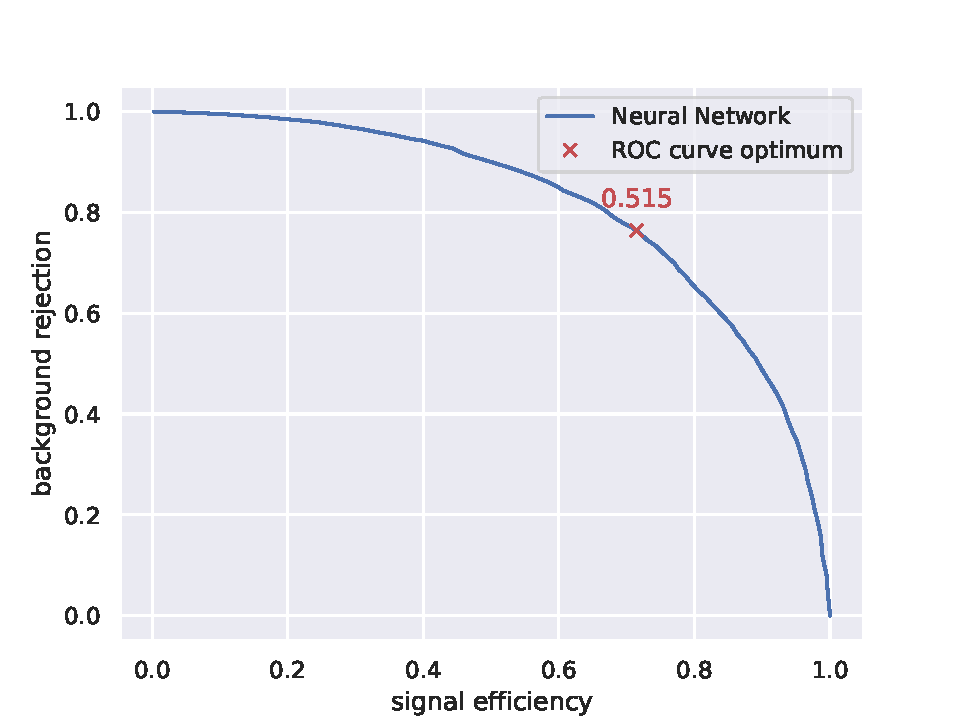
\includegraphics[width=0.5\textwidth]{Plots/ROC-Curve-fullt.pdf}
    \caption{ROC-Curve of the neural network with the point of maximumized signal efficiency and backgrund rejection.}
    \label{fig:rocfull}
\end{figure}

